\documentclass[../main.tex]{subfiles}

\begin{document}

\onehalfspacing

En esta sección se muestra el procedimiento de la generación de  las redes usadas en el trabajo. Asimismo, se presentan los supuestos principales que llevaron a la modelación utilizada.

Se presentan dos tipos de redes: por un lado, se modela la dinámica total de los usuarios comunicantes en todo el periodo de tiempo  observado; por otro lado, se modela  la dinámica de los usuarios antes de la hora pico o el momento de explosividad. 


\begin{table}[h!]
    \caption{Las 10 tendencias más importantes respecto a la cantidad de \textit{tweets} recabados. }
    \centering
    \begin{tabular}{lc}
\toprule
             Tendencia &  Cantidad de \textit{tweets} \\
\midrule
                 \textit{\#oomf} &              363,518 \\
                   \#\textit{np} &              158,608 \\
                   \#\textit{nf} &              128,920 \\
                   \textit{\#ff} &              123,875 \\
       \textit{\#teamfollowback} &               83,064 \\
              \textit{\#bahrain} &               59,277 \\
                   \textit{\#rt} &               51,735 \\
 \textit{\#thoughtsduringschool} &               50,927 \\
                 \textit{\#yolo} &               50,256 \\
             \textit{\#dearoomf} &               40,894 \\
              \textit{\#retweet} &               39,097 \\
                  \textit{\#lrt} &               35,357 \\
                   \textit{\#nw} &               35,323 \\
               \textit{\#taurus} &               35,309 \\
                   \textit{\#lt} &               32,226 \\
\bottomrule
\end{tabular}

    \label{tab:metodologia_10tendenciasmasimportantes}
\end{table}




Cabe mencionar que la modelación se hace con el fin de analizar un comportamiento específico en la dinámica de comunicación de los usuarios en función de la red social. Por lo tanto, el tema inducido por cada nombre de tendencia no se consideró para este trabajo y tampoco se consideró la dependencia entre ellas. Por ejemplo, se tienen tendencias muy relacionadas que registraron una buena actividad de los usuarios; como las tendencias \#ff (acrónimo en inglés de \textit{Follow Friday} ) y \#teamfollowback que refieren a una invitación a seguirse entre los usuarios que participen en la dinámica (ver tabla \ref{tab:metodologia_10tendenciasmasimportantes}). 

% En lo que va de este capítulo, cada vértice en las redes representa un usuario. 

\section{Red de la Dinámica Total}

%Un pequeño resumen de la red
Es una red temporal multicapa (\textit{snapshot}), con dos capas, indexadas por tiempo para cada tendencia. Cada capa estudia un tipo de actividad realizada por los usuarios; en específico, una por \textit{tweets} y otra por \textit{retweets}.  

A esta red de multicapa se nombró como $NC^{\alpha}_{t} (h) $ donde $h$ representa el nombre de la tendencia, $t$ es un periodo de tiempo y $\alpha \in \{T, R\}$ es un índice para la capa de \textit{tweets} y \textit{retweets} respectivamente. 

% En este sentido, $NC^{T}_{t} (h) $ es una red temporal que estudia las actividades de los \textit{Tweets} y $NC^{R}_{t} (h) $ es una red temporal que estudia la actividad de los \textit{retweets}. 

Para la explicación de la construcción de cada una de las capas, se fijó un periodo de tiempo $t$. 
Las capas se construyeron de la siguiente forma:

%Siguen ---> seguían
\begin{itemize}
    \item $NC^{T}_{t}(h)$ es una red no dirigida que representó la dinámica de los \textit{tweets} en la red social de los primeros adoptadores o usuarios. 
    
    En específico, el usuario $A$ realizó un \textit{tweet} en el periodo de tiempo $t$. Se tiene que $A$ y $B$ se seguían mutuamente. Entonces, se definió el enlace $(A,B)$. Cabe recalcar que bastaba con que uno de los dos haya hecho una interacción (\textit{tweet}) para que se generara este mismo enlace en la red.
    
    \item $NC^{R}_{t}(h)$ es una red dirigida que representó la dinámica de los \textit{retweets} en la red social de los primeros usuarios.
    
    Es decir, el usuario $A$ realizó un \textit{tweet} y  un usuario $B$ realizó un \textit{retweet} al \textit{tweet} de $A$ en el periodo de tiempo $t$. Entonces, el enlace $(A,B)$ pertenecía en la red. 
\end{itemize}

En la figura \ref{fig:rep_network_model} se observa una pequeña representación de este modelo. Se hizo referencia a $NC(h) = \cup_{t} NC_{t}(h)$ como la dinámica total de la tendencia $h$. 




%Algunos supuestos y consideraciones de la red. (Supuestos y posibles complicaciones) 
Cabe recalcar que esta red multicapa estaba indexada por tiempo. Es decir, se discretizó la serie de tiempo en intervalos fijos de tiempo. Para este trabajo, la discretización se realizó por intervalos de tiempo de una hora. Esta elección, principalmente, se fundamenta para dar un seguimiento a la cadena de comunicación generada por los usuarios. Dicha cadena no se esperaba con un comportamiento fijo entre usuarios [\cite{Miritello2013}]; por un lado, si el periodo de tiempo era muy corto, se perdía el seguimiento por el alto detalle de análisis; por otro lado, si este periodo era muy largo, se volvía a perder por la gran escala del mismo al no saber de donde nació el \textit{tweet} inicial. Al tratar diversas longitudes de tiempo, se optó el intervalo de tiempo de una hora como el más significativo.








\begin{figure}
    \centering
    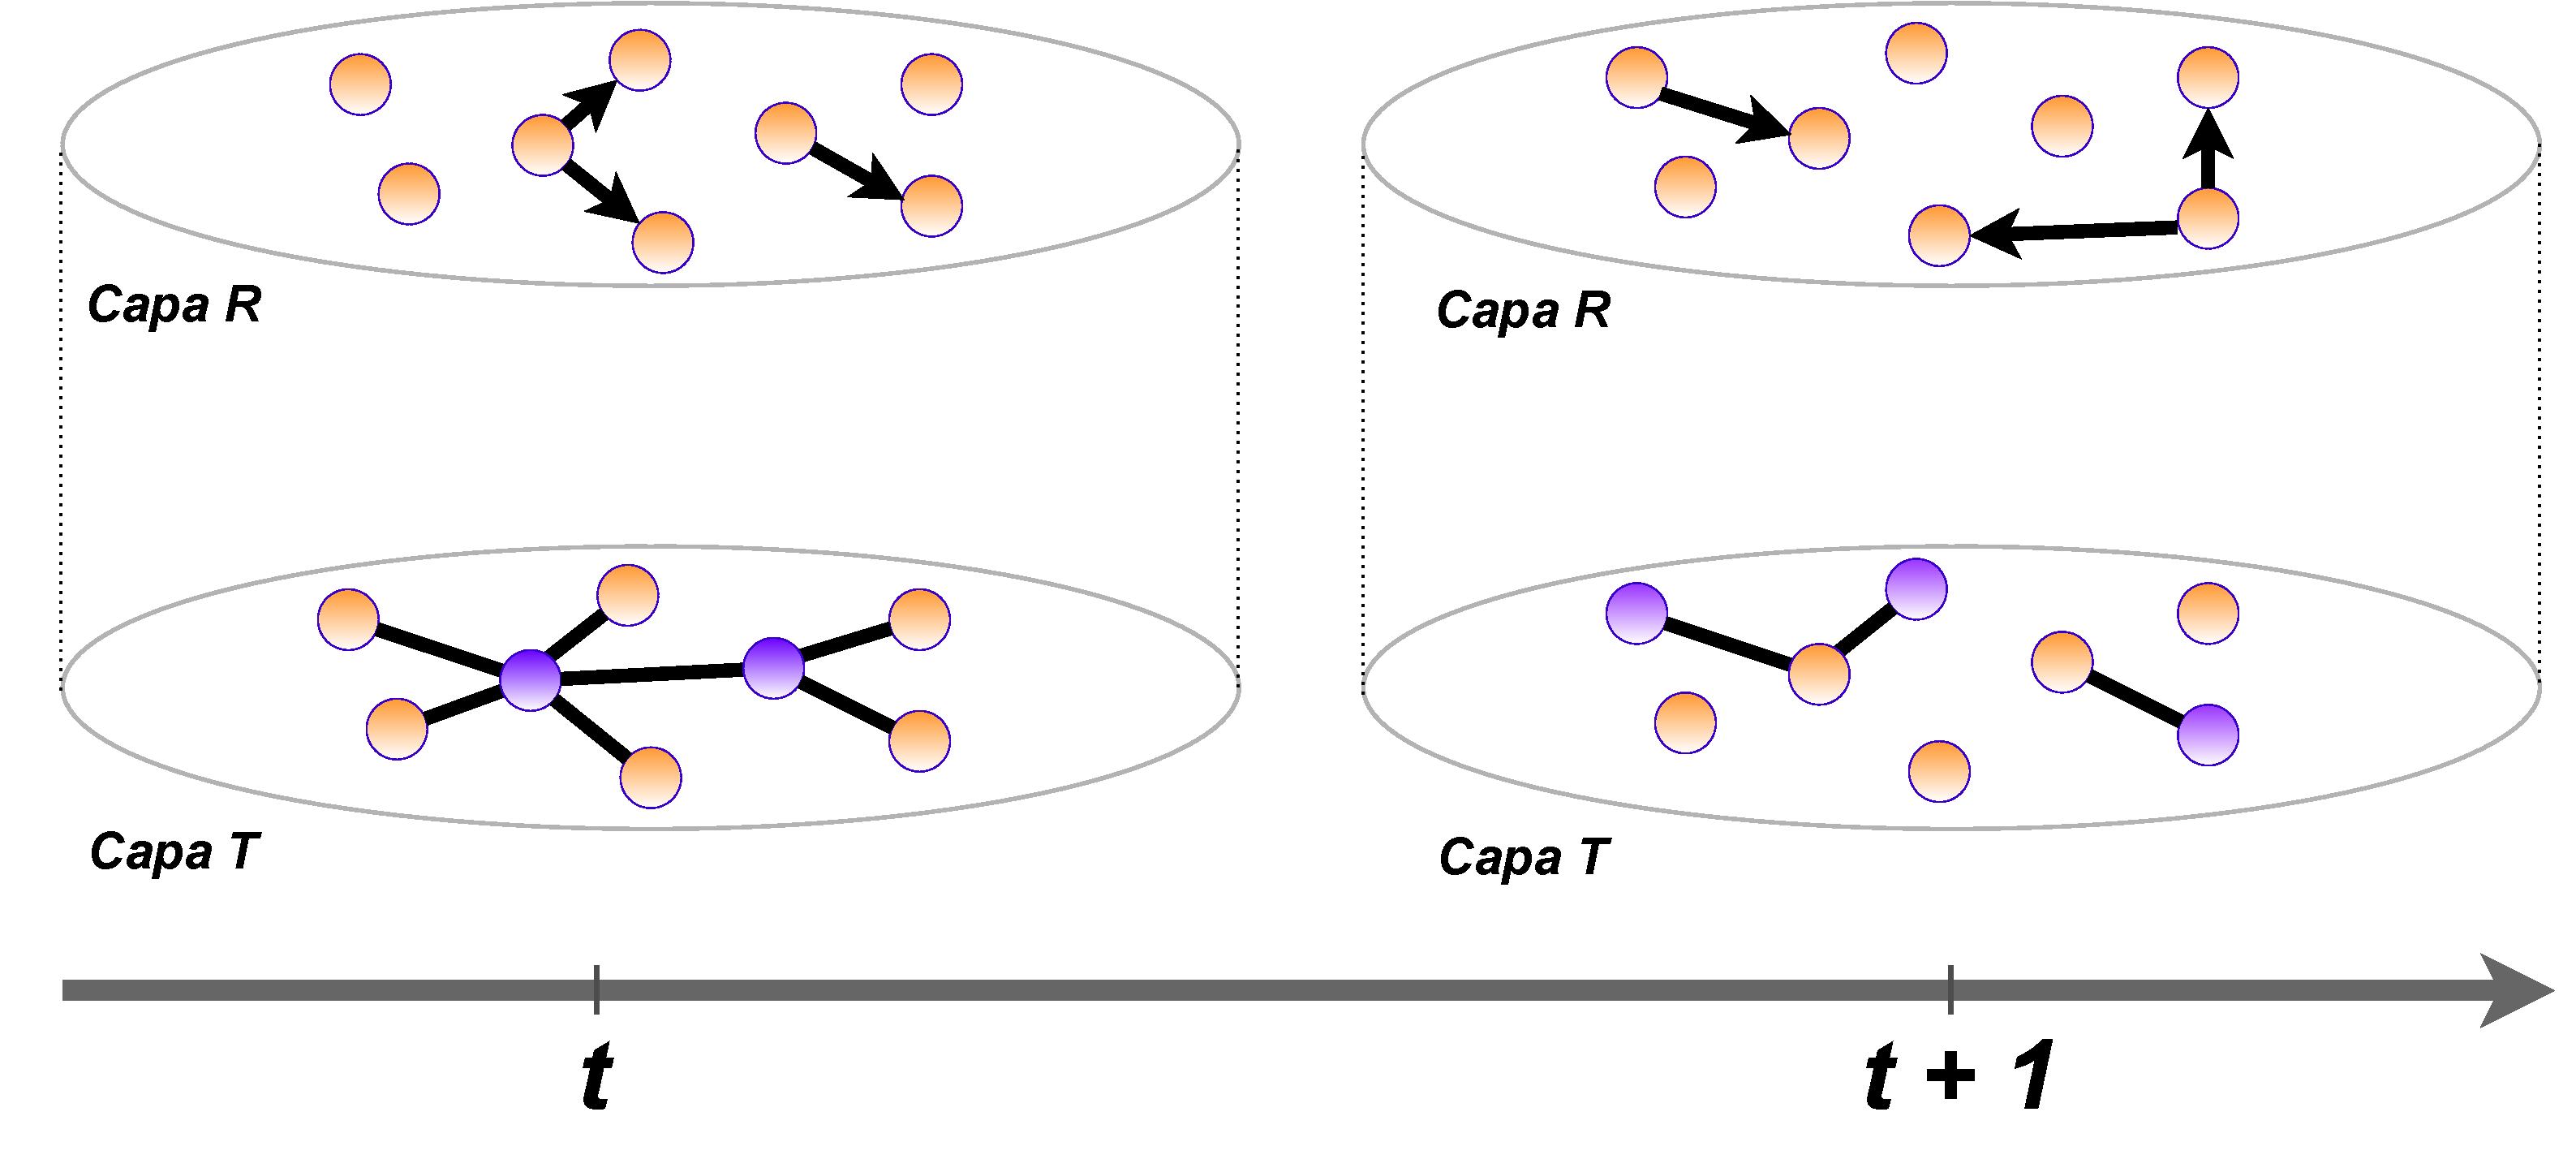
\includegraphics[scale = 0.27]{images/metodologia_multiplexnetwork.drawio.pdf}
    \caption{Ejemplo sencillo de la red $NC^{\alpha}_{t} (h)$ para alguna tendencia de nombre $h$.  Los nodos en color morado representan a los primeros adoptadores de la tendencia. Nótese que no hay enlaces entre capas.}
    \label{fig:rep_network_model}
\end{figure}



% Con base en los modelos presentados en \cite{Model_Pramanik2017, Model_Fabrega_regresion,Model_retweets_inproceedings,D_weng2014predicting}, se presentan los siguientes modelos para abarcar varias necesidades.  Esta modelación se basa en redes temporales, donde cada tiempo $t$ representa un periodo de tiempo. 


\section{Red Pre-Explosividad.}

Es una red no dirigida inducida por los usuarios que adoptaron la tendencia momentos antes del comportamiento explosivo. A esta red se definió como $\G{h}$ donde $h$, siguiendo la notación antes vista, es una tendencia.

A continuación, se presentará el procedimiento explícito de la construcción de esta red. De manera formal y para seguir la notación, sea $G(V,E)$ la red social inicial de todos los usuarios registrados. Cabe recordar que $(a,b) \in E$ si y sólo si $a$ y $b$ se seguían mutuamente. 

El proceso que se menciona en las siguientes líneas se repetirá por cada una de las tendencias. Como en la red anterior, se discretizó la serie de tiempo de la cantidad de \textit{tweets} en intervalos de longitud de 25 minutos. En términos sencillos, se generó la red a partir de la red inducida por los verdaderos primeros comunicantes, Hde manera formal, sea $\left\{ \tau_{i} \right\}_{i=0}^{n}$ el conjunto de dichos intervalos. Sea $\tau_{j}$ el intervalo de tiempo donde ocurrió la mayor cantidad de \textit{tweets} de la tendencia $h$. El conjunto de intervalos de interés es $T = \left\{ \tau_{i} \right\}_{i=\max(j - 404,0)}^{\min(j+404,n)}$. Esto último fue con el fin de obtener un análisis máximo de 14 días. Al cambiar los índices de este último conjunto como $T = \left\{ t_{i} \right\}_{i = 0}^{k}$. 
Sea $U_{t_i}$ el conjunto de usuarios que \textit{tweetearon}, al menos una vez, en el periodo de tiempo $t_i$. Por lo que $U_T = \bigcup_{i = 0}^{k} U_{t_i} $ es el conjunto de todos los usuarios que participaron en el intervalo de interés $T$. 

Sea $\Gamma(X)$ la función que devolvía el conjunto de vecinos del conjunto $X$. Se definió la siguiente recursión $\Gamma^{p}(X) = \Gamma(\Gamma^{p-1}(X)) $ con $\Gamma^{0}(X) = X $ para un $p$ entero positivo. Se definió $\mathcal{E} = \bigcup_{p = 0}^{l} \Gamma^{p}(U_T)$ donde $l$ sería el entero máximo tal que $\left| \mathcal{E} \right| \leq 20,000$. La elección de limitar a 20,000 nodos se hizo para que la comunidad partícipe de nodos representara entre el 10 y 20 por ciento de la red. Para finalizar, $\G{h}$ era igual a la subred inducida por los nodos $\mathcal{E}$. 

% Cabe recalcar que esta última red permitió visualizar las comunidades perdidas a sólo considerar la primera vecindad como en el caso de la red $NC^{T}(h)$. 
% % En el gráfico \ref{fig:nueva_Gl} podemos ver el ejemplo de esta nueva red.


Esta  red se definió para analizar la interacción de los usuarios que verdaderamente realizaron, al menos, un \textit{tweet} en una aproximación a la red social de la que pertenecían; con ello, ver este comportamiento desde las posibles comunidades iniciales.
% , así como algunas diferencias en las métricas usuales de centralidad.
En resumen, se extiendió la red social generada por los usuarios que \textit{tweetearon} hasta un límite de usuarios por cuestiones computacionales. 

La principal justificación y diferencia con la red en la sección anterior es la escala. Por un lado, la red social que abarcaba a los partícipes en el intervalo de una hora donde hubo la mayor interacción (como se definió $NC_{t^{*}}^{T}(h)$ donde $t^{*}$ es el intervalo de tiempo donde hubo mayor interacción) tenía la sutileza en eliminar a los verdaderos pioneros de la tendencia así como en la cantidad de veces que realizan dicha acción.
Esto claramente se puede apreciar en el gráfico \ref{fig:introduccion_comportamientprevio}. %\ref{fig:examplecomportamiento} 
Por otro lado, era necesario escalar la red para abstraer la idea de \textit{usuarios comprometidos} [\cite{West2014}] en distintas comunidades y ver en qué \textit{capa} tenían una interacción clave. Dicha modelación tiene un argumento similar al comportamiento de los sismos para caracterizar comportamientos endógenos y exógenos \cite{Klimek2011_comportamientoend}. 

% Más aún, a sabiendas que muchas de las interacciones iniciales ocurrieron en comunidades \textit{a priori} disconexas, pero con un comportamiento comprometido \cite{D_weng2014predicting} y, justo en el momento de mayor interacción, muchas de las métricas de centralidad parecieran incremetarse y tomar mayor significancia \cite{Chng2015_bottom-up}. 


%-------------------------------------------
% Lo que le sigue no me interesa. 
%-------------------------------------------








% \begin{figure}[h!]
%     \centering
%     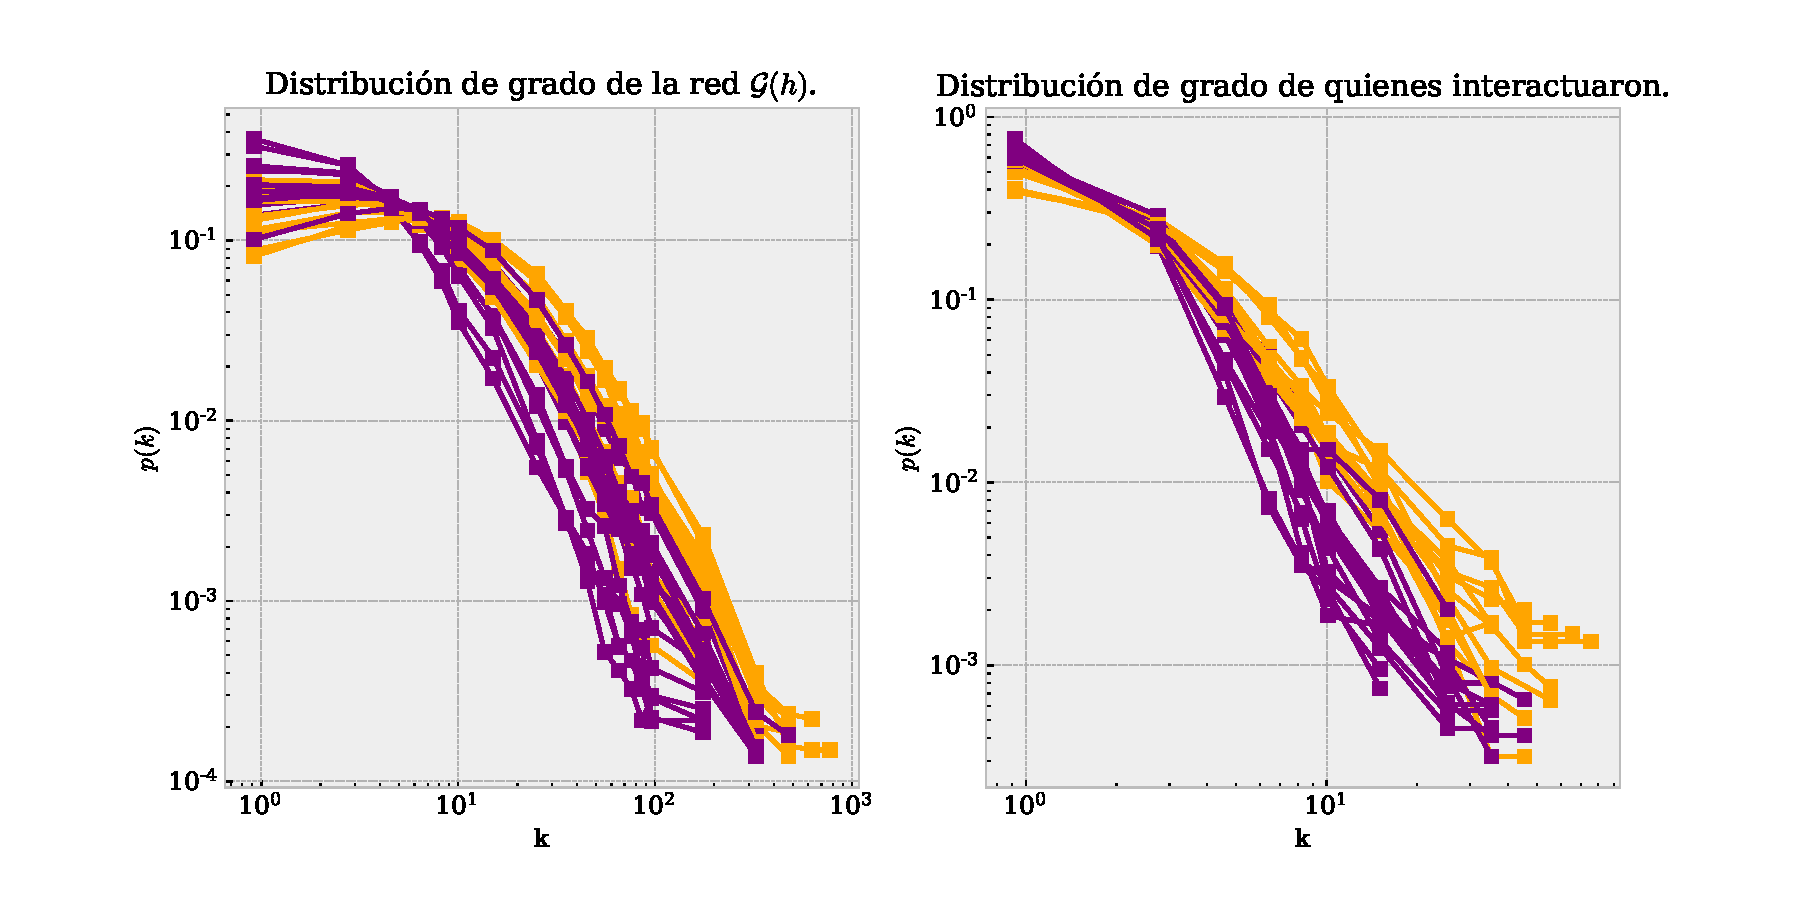
\includegraphics[scale = 0.52]{images/metodologia_differencesNetworks.pdf}
%     \caption{Distribución de grado de la red $\G{h}$. Del lado izquierdo, podemos ver la red $\G{h}$ y del lado derecho del gráfico podemos a la subred inducida por lo nodos que \textit{tweetearon} alguna vez. Las curvas color morado están asociada a una tendencia con comportamiento explosivo. Notemos que la pendiente es inferior en las tendencias con comportamiento explosivo.}
%     \label{fig:qweqw}
% \end{figure}


\section{Datos e Implementación.}

La base de datos utilizada en este trabajo fue recabada por el Centro de Investigación de Redes y Sistemas Complejos (\href{https://cnets.indiana.edu/about/}{CNetS}) [\cite{D_Weng2013, D_weng2014predicting}].  


Esta base cuenta con, aproximadamente, 500 MB de información. La información es un compendio de varios seguimientos del portal \textit{Twitter} desde el 24 de marzo de 2012 al 26 de abril de 2012. Cabe recalcar que, por las políticas de privacidad de \textit{Twitter}, todos los usuarios que aparecen tienen un identificador único y diferente a su cuenta original; por lo que no es posible hacer búsqueda de dicha cuenta a través de otras paqueterías u obtener una información sobre los usuarios u obtener explícitamente lo que se haya publicado. Hay 14,273,311 usuarios recabados con 1,345,913 de tendencias y 12,054,205 $tweets$ en total.

Para esta modelación, se realizó una limpieza de toda la base. El primer filtro fue considerar sólo aquellas que tuvieran, al menos, 4000 \textit{tweets} registrados. Así, se analizaron únicamente 143 tendencias. 

Los modelos que se mencionaron se implementaron con el lenguaje de programación \href{https://www.python.org/}{Python}; haciendo uso de diversas paqueterías, entre ellas \href{https://networkx.org/}{NetworkX} para el trato y manipulación de las redes y de \href{https://networkit.github.io/}{NetworkIt} para el cálculo de diversas métricas. La implementación se encuentra alojada en el repositorio \href{https://github.com/ErickMM98/NetworkAnalysis_TwitterTrends}{Github}.


\end{document}